\documentclass{beamer}
\beamertemplatenavigationsymbolsempty
\usecolortheme{beaver}
\setbeamertemplate{blocks}[rounded=true, shadow=true]
\setbeamertemplate{footline}[page number]
%
\usepackage[utf8]{inputenc}
\usepackage[english,russian]{babel}
\usepackage{amssymb,amsfonts,amsmath,mathtext}
\usepackage{subfig}
\usepackage[all]{xy} % xy package for diagrams
\usepackage{array}
\usepackage{multicol}% many columns in slide
\usepackage{hyperref}% urls
\usepackage{hhline}%tables
% Your figures are here:
\graphicspath{ {fig/} {../fig/} }

\fontsize{10}{12}\selectfont

%----------------------------------------------------------------------------------------------------------
\title[\hbox to 56mm{Порождение признаков}]{Порождение признаков \\ в задачах классификации и прогнозирования}
\author[Н.\,П. Ивкин]{Никитина Мария Александровна}
\institute{Московский физико-технический институт}
\date{\footnotesize
\par\smallskip\emph{Курс:} Автоматизация научных исследований\par (практика, В.\,В.~Стрижов)/Группа 874
\par\smallskip\emph{Эксперт:} О.\,Н.~Петров
\par\smallskip\emph{Консультант:} Ш.\,Л.~Фоменко
\par\bigskip\small 2021}
%----------------------------------------------------------------------------------------------------------
\begin{document}
%-----------------------------------------------------------------------------------------------------
\begin{frame}{Автоматическое выделение терминов в тематическом моделировании}
\begin{columns}[c]
\column{0.4\textwidth}
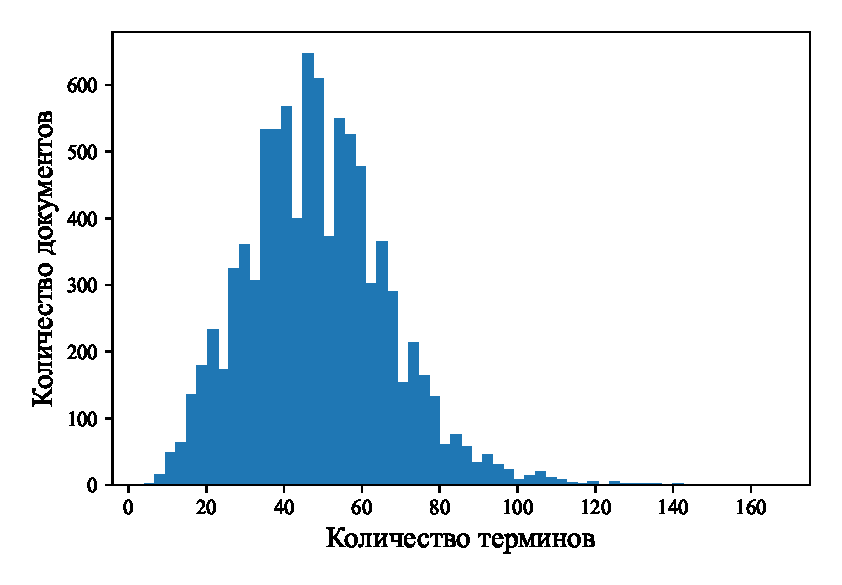
\includegraphics[width=1.0\textwidth]{Pictures/Statistics_1.eps}
\column{0.6\textwidth}
\begin{small} Для решения задачи используется алгоритм выделения коллокаций TopMine в сочетании с модульной технологией тематического моделирования. \end{small}
    
\end{columns}

\bigskip
\[P = \Phi\Theta\]
\end{frame}
%----------------------------------------------------------------------------------------------------------
\end{document} 